\documentclass[]{IEEEtran}
% some very useful LaTeX packages include:
%\usepackage{cite}      
\usepackage{graphicx}   
\usepackage{subfigure} 
\usepackage{url}       
\usepackage{amsmath}    
\usepackage{caption2}
% Your document starts here!
\begin{document}

% Define document title and author
	\title{Weekly Report}
	\author{Adviser: Prof. Yang Wen \\Student: Cheng Wensheng\\ Period: 2018.5.11-5.18
	}
	\markboth{Visual Information Processing Group}{}
	\maketitle

% Write abstract here
\begin{abstract}
	This week I mainly put my effort on finding materials of SAR image contest and reading a new paper called StarGAN, which is accepted by CVPR 2018 as oral paper. 
\end{abstract}

% Each section begins with a \section{title} command
\section{Paper reading}
	% \PARstart{}{} creates a tall first letter for this first paragraph
	\PARstart{R}{ecent} studies have shown remarkable success in image-to-image translation for two domains. However, existing approaches have limited scalability and robustness in handling more than two domains, since different models should
	be built independently for every pair of image domains. To
	address this limitation, they propose StarGAN, a novel and
	scalable approach that can perform image-to-image translations
	for \textbf{multiple domains using only a single model.} Overall, the contributions are as follows:
	\begin{itemize}
		\item They propose StarGAN, a novel generative adversarial
		network that learns the mappings among multiple domains	using only a single generator and a discriminator, training effectively from images of all domains.
		\item They demonstrate how we can successfully learn multidomain	image translation between multiple datasets by utilizing a mask vector method that enables StarGAN
		to control all available domain labels.
		\item They provide both qualitative and quantitative results on facial attribute transfer and facial expression synthesis tasks using StarGAN, showing its superiority over
		baseline models.
	\end{itemize}

	The author did complete experiments to show StarGAN's priority to other StoA models, including DIAT, CycleGAN, IcGAN,etc. This is a really heuristic work which I believe will influence following studies a lot. Fig.~\ref{fig:mp} is the Comparison between cross-domain models and StarGAN. Fig.~\ref{fig:ss} is the StarGAN training strategy.
	

% Main Part

\newpage
\begin{figure}[!hbt]
%		 Center the figure.
		\vspace{1.7cm}
%		\hspace{50cm}
		\begin{center}
			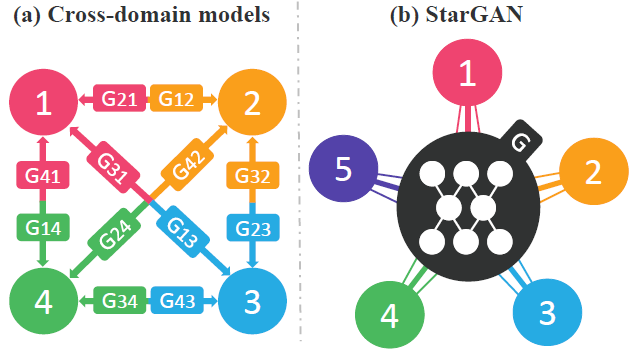
\includegraphics[width=\columnwidth]{ff}
				%		 Create a subtitle for the figure.
			\caption{Comparison between cross-domain models and StarGAN}
			\label{fig:mp}
		    \hspace{0.5cm}
			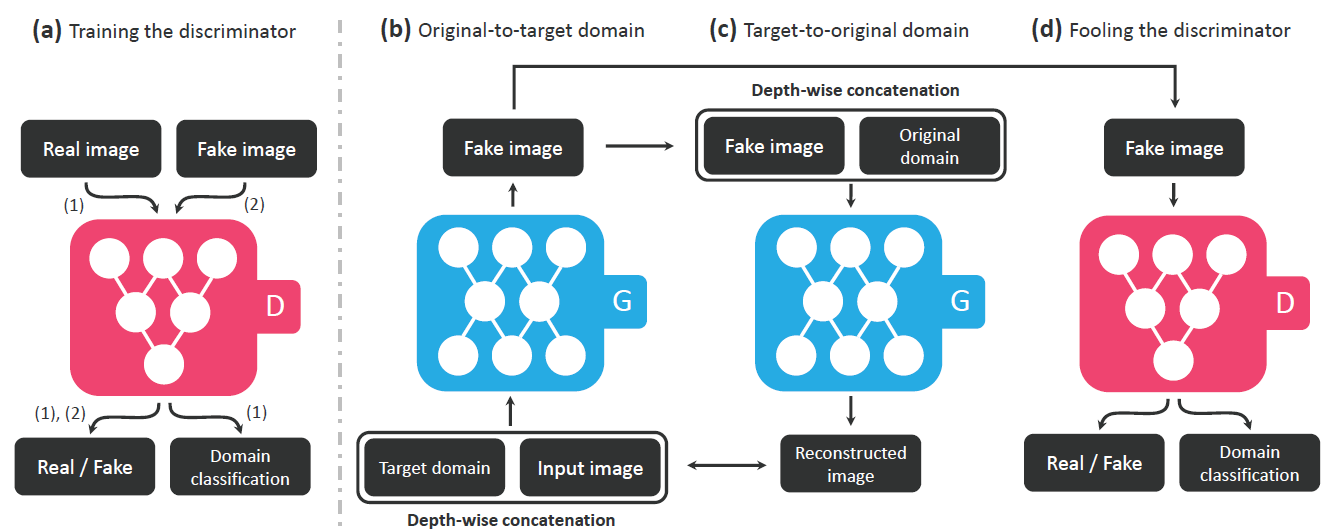
\includegraphics[width=\columnwidth]{ts}
				%Create a subtitle for the figure.
			\caption{StarGAN training strategy}
			\label{fig:ss}
		\end{center}
	\end{figure}

% Now we need a bibliography:
%\begin{thebibliography}{5}
%
%	%Each item starts with a \bibitem{reference} command and the details thereafter.
%	\bibitem{HOP96} % Transaction paper
%	J.~Hagenauer, E.~Offer, and L.~Papke. Iterative decoding of binary block
%	and convolutional codes. {\em IEEE Trans. Inform. Theory},
%	vol.~42, no.~2, pp.~429–-445, Mar. 1996.
%
%	\bibitem{MJH06} % Conference paper
%	T.~Mayer, H.~Jenkac, and J.~Hagenauer. Turbo base-station cooperation for intercell interference cancellation. {\em IEEE Int. Conf. Commun. (ICC)}, Istanbul, Turkey, pp.~356--361, June 2006.
%
%	\bibitem{Proakis} % Book
%	J.~G.~Proakis. {\em Digital Communications}. McGraw-Hill Book Co.,
%	New York, USA, 3rd edition, 1995.
%
%	\bibitem{talk} % Web document
%	F.~R.~Kschischang. Giving a talk: Guidelines for the Preparation and Presentation of Technical Seminars.
%	\url{http://www.comm.toronto.edu/frank/guide/guide.pdf}.
%
%	\bibitem{5}
%	IEEE Transactions \LaTeX and Microsoft Word Style Files.
%	\url{http://www.ieee.org/web/publications/authors/transjnl/index.html}
%
%\end{thebibliography}

% Your document ends here!
\end{document}